%%%%%%%%%%%%%%%%%%%%%%%%%%%%%%%%%%%%%%%%%%%%%%%%%%%%
\documentclass[12pt]{report}
\usepackage[a4paper, margin=1in]{geometry}
\usepackage{graphicx}
\usepackage{url}
\usepackage{tikz}
\usepackage{eso-pic}
\usepackage{booktabs}
\usepackage{longtable}
\usepackage{parskip}
\usepackage[hidelinks]{hyperref}
\usepackage[round]{natbib}
\usepackage{ragged2e}
\usepackage{titlesec}
\usepackage{setspace}
\usepackage{indentfirst}
\usepackage[none]{hyphenat}\sloppy
\usepackage[toc,titletoc]{appendix}
\usepackage{graphicx}
%%%%%%%%%%%%%%%%%%%%%%%%%%%%%%%%%%%%%%%%%%%%%%%%%%%%


%%%%%%%%%%%%%%%%%%%%%%%%%%%%%%%%%%%%%%%%%%%%%%%%%%%%
\newcommand{\papertitle}{Language Requirements in Berlin's Job Market: A Comparison of International Image and Labor Market Practice}
\newcommand{\researchquestion}{To what extent does Berlin's international and English-friendly reputation reflect the linguistic requirements of its labor market for non-German speaking professionals?}
\newcommand{\student}{Ali M Abdou, Chakib Khemaissia, Nibras H Nathu, Omid Karimi}
\newcommand{\module}{B124 Academic Writing and Research Methods}
\newcommand{\supervisor}{Vahab Esfandani}
\newcommand{\modleader}{Prof. Dr. Sara Ramzani}
\newcommand{\submissiontime}{SS0325}
%%%%%%%%%%%%%%%%%%%%%%%%%%%%%%%%%%%%%%%%%%%%%%%%%%%%


%%%%%%%%%%%%%%%%%%%%%%%%%%%%%%%%%%%%%%%%%%%%%%%%%%%%

\hypersetup{
	pdftitle={\papertitle},
	pdfsubject={B124D Academic Writing and Research Methods @ GISMA UNIVERSITY OF APPLIED SCIENCES},
	pdfauthor={\student},
	pdfkeywords={Language Requirements, Berlin, Job Market, International Image, Labor Market, English, German, Employment, Globalization, Expatriates, Immigrants}
}


\titleformat{\chapter}[hang]{\normalfont\bfseries\fontsize{14}{0}\selectfont}{\thechapter.\quad}{0pt}{\normalfont\bfseries\fontsize{14}{0}\selectfont}
\titlespacing*{\chapter}{0pt}{12pt}{0pt}

\titleformat{\section}[hang]{\normalfont\bfseries\fontsize{12}{0}\selectfont}{\thesection.\quad}{0pt}{\normalfont\bfseries\fontsize{12}{0}\selectfont}
\titlespacing*{\section}{0pt}{21pt}{0pt}

%%%%%%%%%%%%%%%%%%%%%%%%%%%%%%%%%%%%%%%%%%%%%%%%%%%%


%%%%%%%%%%%%%%%%%%%%%%%%%%%%%%%%%%%%%%%%%%%%%%%%%%%%
\renewcommand\maketitle{
	{
		\center
		\begin{tikzpicture}[remember picture, overlay]
			\node[opacity=0.2,inner sep=0pt] at (current page.south) [yshift=5cm]{
				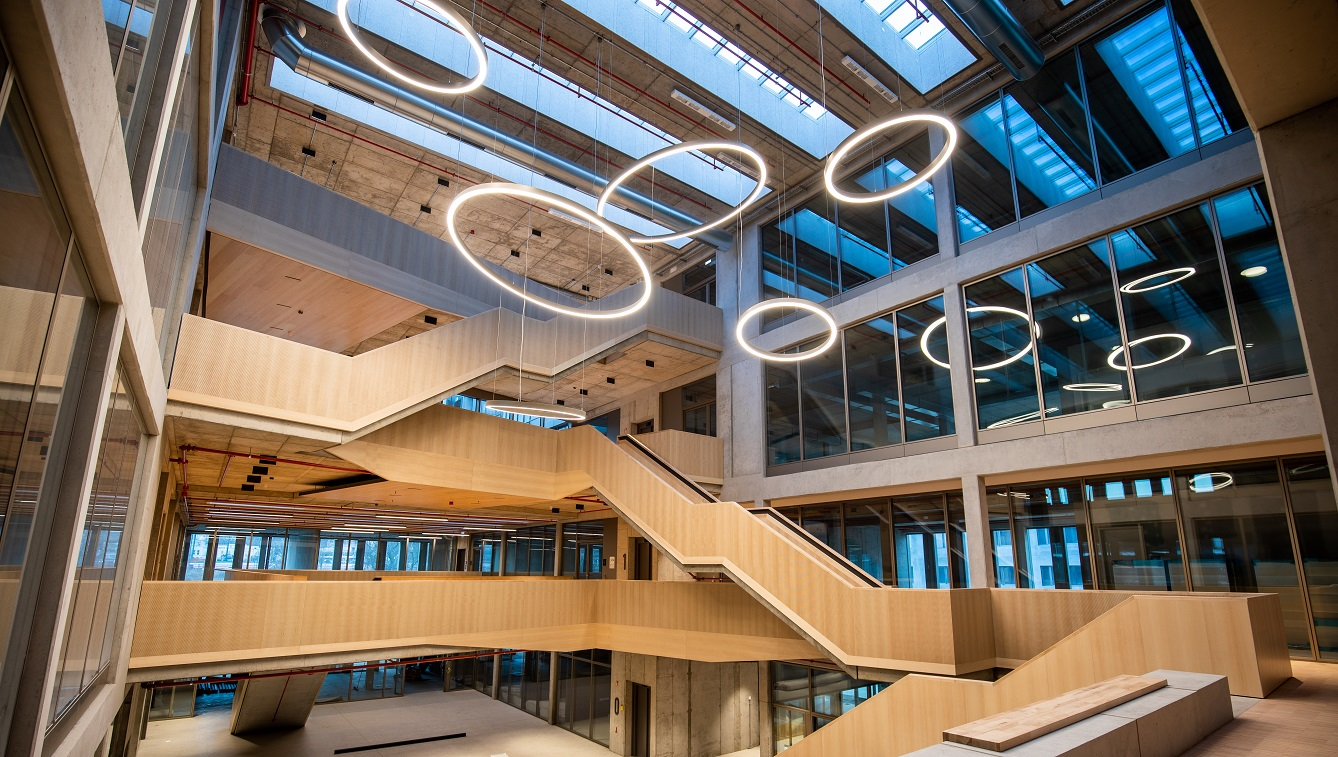
\includegraphics[width=\paperwidth, height=\paperheight, keepaspectratio]{attachments/campus}
			};
		\end{tikzpicture}
		
\includegraphics[width=0.6\textwidth]{attachments/logo}\par
		{\scshape\LARGE\bf Gisma University of Applied Sciences \par}
		\vspace{2cm}
		\rule{\linewidth}{0.5mm}\par
		{\huge\bfseries\papertitle\par}
		\rule{\linewidth}{0.5mm}\par
		\vspace{0.2cm}
		{\Large\student\par}
		\vspace{0.2cm}
		{\large\module\par}
		\vspace{10.25cm}
		{\large\submissiontime\par}
		\thispagestyle{empty} 
		\newpage
	}
}

\newcommand\makesubtitle{
	{
		\center
		
\includegraphics[width=0.4\textwidth]{attachments/logo2}\par
		{\scshape\Large\bf Gisma University of Applied Sciences \par}
		\vspace{0.8cm}
		\raggedright
		\rule{\linewidth}{0.3mm}\par
		\vspace{0.8cm}
		\normalsize
		Paper Title \par
		\textbf{\papertitle}\par
		\vspace{0.8cm}
		Research Question \par
		\textbf{\researchquestion}\par
		\vspace{0.8cm}
		Collaborative report by:  \par
		\begin{tabular}{@{}l@{\hspace{3em}}l@{\hspace{3em}}l}
			\bf\normalsize{Ali Mohamed Abdou} & GH1033452 & alimohamed.fathi@gisma-student.com \\[0.6ex]
			\bf\normalsize{Chakib Khemaissia} & GH1029909 & chakib.khemaissia@gisma-student.com \\[0.6ex]
			\bf\normalsize{Nibras Hassan Nathu} & GH1036309 & nibras.nathu@gisma-student.com \\[0.6ex]
			\bf\normalsize{Omid Karimi} & GH1038348 & omid.karimi@gisma-student.com \\[0.6ex]
		\end{tabular}\par
		\vspace{0.8cm}
		{\normalsize Submitted in  fulfillment of the final assessment for the module\par}
		{\normalsize\bf\module\par}
		\vspace{0.7cm}
		{\normalsize Lecturer\par}
		{\normalsize\bf\supervisor\par}
		\vspace{0.7cm}
		{\normalsize Module Leader\par}
		{\normalsize\bf\modleader\par}
		\vspace{0.7cm}
		{\normalsize Submission Quarter\par}
		{\bf\large\submissiontime\par}
		\center
		\thispagestyle{empty}
		\newpage
	}
}

\begin{document} 
%%%%%%%%%%%%%%%%%%%%%%%%%%%%%%%%%%%%%%%%%%%%%%%%%%%%


%%%%%%%%%%%%%%%%%%%%%%%%%%%%%%%%%%%%%%%%%%%%%%%%%%%%
\pagestyle{plain}
\pagenumbering{roman}
\newgeometry{margin=2cm}\maketitle
\makesubtitle
\chapter*{}
\vspace{17cm}
\hfill\parbox{8cm}{
\raggedleft
	\textit{We confirm that this collaborative report is our own work and that we have documented all sources and materials used.}\par 
	\vspace{1em}
	Berlin, 24 June 2025

	\vspace{3em}
	{\footnotesize Word Count: 3,285}
}
\thispagestyle{empty} \restoregeometry\justifying
\pdfbookmark[1]{Abstract}{abstract}
\chapter*{Abstract} 
\phantomsection
\noindent\setstretch{1.2}This study examines the disparity between Berlin’s well-established international reputation as an English-friendly city and the actual language requirements that non-German-speaking professionals encounter in the labor market. By employing a mixed-methods approach, the research combines an analysis of current job listings from various industries with primary survey data collected from international students and expatriates residing in the Berlin Metropolitan Area. The findings reveal a significant discrepancy: although the city is perceived as an accessible hub for English speakers, most full-time job listings still require proficiency in German. The survey results reinforce this observation, indicating that many non-German-speaking professionals experience rejection due to insufficient German language skills. At the same time, the perception of an English-only job market is considerably higher than what is observed. The study concludes by emphasizing that having German language skills remains a significant hurdle to employment for non-German speakers in Berlin. It advocates for a more accurate representation of the city’s language job market requirements to help manage expectations and support improved professional integration.
\tableofcontents 
%%%%%%%%%%%%%%%%%%%%%%%%%%%%%%%%%%%%%%%%%%%%%%%%%%%%

\doublespacing

%%%%%%%%%%%%%%%%%%%%%%%%%%%%%%%%%%%%%%%%%%%%%%%%%%%%
\clearpage
\pagenumbering{arabic}
\setlength\parindent{20pt}
\begingroup\let\clearpage\relax
\titlespacing*{\chapter}{0pt}{0pt}{0pt}

\chapter{Introduction}

intro \citep{placeholder}

\titlespacing*{\chapter}{0pt}{12pt}{0pt} \vspace{12pt}
\chapter{Literature Review}

lit rev \endgroup
\chapter{Methodology}

To address this study’s research question, this paper employs a mixed-method approach comprising primary and secondary research strategies. This will provide a comprehensive perspective on how language impacts employability in Berlin, especially for individuals who are not fluent in German. Additionally, this mixed approach will allow for a relative comparison of secondary works and current-day testimonials as of the summer of 2025.

Primary data was collected via an online survey distributed through university mailing lists, online forums, and social media platforms. The survey was created using Microsoft Office Forms (see Appendix A). It targeted expatriates and international students and was conducted anonymously with informed consent provided through a data protection disclaimer (datenschutzhinweis) written in both German and English. Additionally, the survey includes sections on demographics, academic background, employment preferences, language skills, and job search experience. Thus, the survey enables the collection of both statistical trends and subjective perceptions regarding the role of language in Berlin’s job market.

Primary research aids and benefits this paper by ensuring contemporary data is included. The survey used in this paper allows this research to “avoid unreliable information from outside sources” \citep{Indeed25}. However, primary research comes with its respective challenges \citep{k2024crucial}. The survey conducted in this study was particularly time-consuming and difficult to distribute. Issues arose when convincing individuals to take a few minutes to complete the survey, as many individuals had refused to participate in such a study without an incentive. Also, the sample size was limited due to the difficulty in distributing the survey to the large number of Berlin residents. Some respondents may also downplay the issue of language requirements if they had help from inside their company, or, contrary, where some may exaggerate the issue due to bad experiences during the hiring process.

Secondary data was collected through a content analysis of job listings on platforms like LinkedIn, Indeed, StepStone, and businesses’ direct hiring portals. Said listings include jobs from various industries, including technology, marketing, education, healthcare, customer service, government, and finance. Each job listing was analyzed to determine the language it was posted in, the language requirements listed, the industry, and the industry level. This data helps evaluate how frequently English-friendly positions are advertised, which industries offer such positions, and whether German language skills are a formal prerequisite or an implicit expectation. Notably, this paper does not aim or intend to explore the differences in salaries and job benefits between positions that require unwavering German language skills and positions that require little or no knowledge of the German language.  

Secondary research is a key component of any study, providing nearly unlimited insight into other institutions’ discoveries on a topic. Secondary research is an easy, cheap, and fast method of data collection that does not require “[involvement] in developing complicated data collection methods” \citep{Nasrudin25}. Particularly with the rise of generative AI tools, such as ChatGPT, secondary research has become increasingly simple; it merely requires a quick prompt instructing an AI tool to search the internet for sources on any given topic. Additionally, secondary research is more varied, allowing a surplus of data to be used in comparison. However, secondary research comes with its respective disadvantages. For instance, the data may be inaccurate, as no piece can ever be fully verified as authentic. It may also be out-of-date, providing information that no longer applies to the current industry norms and requirements \citep{Nasrudin25}.

\chapter{Results and Discussion}
\vspace{5pt}
\section{Job Listing Analysis}
An analysis of 191 Berlin job listings (see \hyperref[appendix:B]{Appendix~B}) revealed that 75.4\% specified listings required at least conversational German (19.9\% conversational, 55.5\% fluent), while 24.6\% required none. Fifty-two percent of listings were posted in English, 47.1\% in German, and 0.5\% in both. This contrasts with national data indicating that 97\% of jobs require German \citep{Jones25}. While the sample shows a greater presence of English, a significant German barrier persists, challenging Berlin’s perceived friendliness to English speakers.

\subsection{Information Technology}
Of 44 IT listings, 34.1\% needed no German, 25\% required conversational German, and 40.9\% needed fluent German. Sixty-five postings were in English. This sector is English-friendly, with many platforms listing English-speaking roles. Many tech companies foster “English-speaking environments,” creating an English-speaking “bubble”.   

\subsection{Finance}
Of 37 finance listings, 62.2\% required fluent German, 13.5\% conversational German, and 24.3\% no German, with 48.6\% being listed in German. This indicates that finance roles, particularly those involving German regulations, often require German fluency.

\subsection{Healthcare}
Core medical professions require German exams (B2-C2). Primary data shows that roles like `Medizinische Fachangestellte' require fluent German. Bureaucratic tasks are primarily in German. This represents a life-critical language barrier. 

\subsection{Education}
The English teaching market is peculiarly saturated. Certified teachers in public schools require proficiency in fluent German. Primary data shows mixed requirements (33.3\% none, 16.7\% conversational, 50\% fluent), with 70.8\% of listings posted in English.

\subsection{Public Services}
Of 24 public service listings, 58.3\% required fluent German, 12.5\% conversational German, and 29.1\% required none, with 50\% listed in English. Public service roles almost universally require proficiency in German due to the state administration and bureaucracy.   

\subsection{Manufacturing}
Of 23 manufacturing listings, 65.2\% required fluent German, 21.7\% required conversational German, and 13\% required no German proficiency. With 39.1\% of being listed in English and 4.3\% being listed in both languages, this suggests that blue-collar work, such as manufacturing, tends to require proficiency in German for ease of communication.

\subsection{Marketing}
Of 29 listings for marketing, 48.3\% required fluent German, 34.5\% required conversational German, and 17.2\% required none. Forty-eight percent of listings were in English. This suggests that German businesses tend to market primarily to German-speaking consumers, rather than international customers, given that the majority of positions require proficiency in the language.

\section{Survey Findings}
\vspace{5pt}
\subsection{Demographics Language Proficiency, and Perceptions of Respondents}
The survey gathered responses from young professionals and students, primarily aged 18-25 (69\%) and 26-35 (23\%). Most respondents held or were pursuing a bachelor’s degree (54\%), while the remainder held or were working towards a master’s degree (46\%). Many respondents were from Gisma University of Applied Sciences, reflecting the demographics of international students and expatriates. A significant majority (69\%) of participants reported Beginner (A1-A2) proficiency in German, with 15\% having no German skills. Additionally, 73\% were fluent in English, while the remaining 27\% possessed intermediate (B1-B2) English skills.

This linguistic profile, which indicates a highly educated group with strong English but limited German, supports the argument that Berlin attracts English-speaking professionals who are underprepared for the broader German-speaking labor market. Respondents indicated that only a tiny number of job listings did not require German language skills. Sixty-two percent reported that only 0-25\% of job listings in their desired field were posted in English, with 19\% reporting 26-60\%. In further support of the assertion that German is almost always required in the workplace, 42\% stated that German was always required in their field, while 38\% said it was often necessary. This inconsistency between Berlin’s English-friendly reputation and its actual job market outlines the widespread reality for job seekers, creating an imminent employment challenge.


\subsection{Impact of German Language Skills on Job Searches}
Sixty-nine percent of participants reported job application rejections due to insufficient German skills. Only 12\% were able to secure employment without fluency in German, primarily in the hospitality and information technology sectors. Additionally, 31\% were not invited to any interviews, suggesting that language barriers hinder initial screening and indicating limited English-only opportunities. This empirical evidence supports the claim that language proficiency has a significant impact on employment.

Before relocating to Berlin, 50\% of participants believed they could find a job there without speaking German, which aligns with the city’s image. However, when asked if Berlin’s English-friendly reputation accurately reflects the job market, 50\% stated that this was not true at all, while an additional 23\% expressed that it was only slightly true. This stark contrast reveals a significant gap between reputation and reality. Berlin’s marketing creates unrealistic expectations that lead to frustration and dissatisfaction for expatriates and international students.

\section{Analysis}
The study reveals a significant gap between Berlin’s image as an English-friendly city and its labor market realities. Survey respondents report a shortage of English-only job listings (0-25\% for 62\%), aligning with national data indicating that 96-97\% of postings require German proficiency. An 88\% rejection rate due to inadequate German skills highlights the linguistic demands in most sectors. The success rate for non-fluent German speakers demonstrates a labor market where English-only positions are rare. While English suffices in tourism, it is insufficient in traditional industries and public services, which are primarily conducted in German. Despite Berlin’s marketing as an English-friendly city, actual labor market conditions require German proficiency, posing challenges for non-German speakers. A lack of German skills hinders career advancement and income growth. Proficiency is crucial for navigating bureaucracy and internal communication. New residency regulations mandating German proficiency formalize this situation, acting as a socio-economic gatekeeper and relegating non-German speakers to a secondary labor market with limited integration opportunities.

Berlin’s competitive market faces an oversaturation of English-only job openings. Recruiters often seek a “perfect fit,” including one that matches their language preferences. Daily life and administrative tasks remain predominantly German-speaking. Implicit German expectations can lead to rejections, and employers may exhibit statistical discrimination. This often limits qualified international professionals to low-skilled roles, leading to underemployment.

The tech and startup ecosystem offers the best path for English-speaking professionals, particularly in software development and AI. Learning German is vital as it broadens job opportunities and enhances career prospects. Government language courses boost employment opportunities. Berlin presents an English-friendly image but reveals a German-dominated reality, requiring job seekers to adapt their strategies accordingly. Opportunities lie in competitive niches, while the broader market remains inaccessible without German. The focus should be on long-term German language investment and targeted networking to break through barriers and achieve integration. \par

\chapter{Project Closure}

The closure of the project represents the concluding phase of the project lifecycle, encompassing the formal certification of completion, evaluation of outcomes, and verification that deliverables adhere to the mutually agreed-upon standards. Given the intricacy of the CHSR project, the closure process must be executed in a phased and strategic manner to ensure sustainability, compliance, and stakeholder satisfaction.

\section{Closure Criteria}
For each segment, such as the Central Valley IOS, completion is contingent upon the fulfillment of all contractual deliverables (including infrastructure, safety systems, and interoperability), the successful performance testing and commissioning of all systems, and obtaining regulatory approval. A segment shall not be deemed complete unless these three criteria are satisfied. These criteria cannot be prioritized by urgency, as the first pertains to the physical installation of the project, the second concerns safety and operability, and the third involves securing legal approval from state authorities and ensuring compliance with safety, environmental, and technical standards. \par

\section{Acceptance Process}
The acceptance process begins with the Project Management Office issuing formal handover reports to the CHSR authority’s executive board and operations division, indicating that the project is ready for operational review. At the same time, an Operational Readiness Review is conducted to carefully verify that all key components, including sufficient staffing, robust systems, and detailed maintenance plans, are in place and prepared for deployment. The final crucial step is obtaining stakeholder sign-off, which involves securing approval from key stakeholders, including the State of California, the Federal Railroad Administration, and relevant community representatives, especially those in areas heavily affected by eminent domain or construction activities. This process ensures that all concerns are adequately addressed before the project is officially accepted.

\section{Documentation and Archiving}
Any project requires thorough documentation for future research and growth. Fortunately, the CHSR authority is mandated by the State of California’s Legislative Analyst’s Office to submit annual project update reports and business plan updates every 2-4 years (or whenever there is a change to the plan). This requirement will simplify archiving, as by the project’s end, only minor edits will be needed for the latest business plan and project update report to accurately reflect the project’s overall progress. This includes final risk registers, procurement logs, financial records, commissioning records, warranties, legal documents, and stakeholder agreements. Additionally, all documentation must be stored in a centralized digital repository to comply with California’s Public Records Act (California Government Code, § 6250 et seq.).

\section{Conclusions and Transitions}
Project reviews shall be conducted to assess schedule compliance, cost deviations, the efficacy of stakeholder engagement strategies, contractor and supplier performance, and the effectiveness of risk management. These insights shall offer a prospective outlook for CHSR segments and other significant infrastructure endeavors within California. Upon completion, responsibilities will be transferred from the Project Management Office to the Operations and Maintenance Division, which will oversee the daily service operations, ongoing maintenance, and user feedback collection of the CHSR. Staff recruitment, training, and onboarding procedures should commence approximately six months prior to the project’s completion to facilitate a seamless transition. \par
\clearpage 
%%%%%%%%%%%%%%%%%%%%%%%%%%%%%%%%%%%%%%%%%%%%%%%%%%%%


%%%%%%%%%%%%%%%%%%%%%%%%%%%%%%%%%%%%%
\raggedright
\phantomsection
\renewcommand{\bibname}{References}
\addtocounter{chapter}{1}\addcontentsline{toc}{chapter}{\thechapter\ \ \bibname} 
\bibliographystyle{agsm}
\bibliography{attachments/bibliography}
%%%%%%%%%%%%%%%%%%%%%%%%%%%%%%%%%%%%%%%%%%%%%%%%%%%%


%%%%%%%%%%%%%%%%%%%%%%%%%%%%%%%%%%%%%%%%%%%%%%%%%%%%
\clearpage \justifying
\addtocounter{chapter}{1}\addcontentsline{toc}{chapter}{\thechapter\ \ Appendices} 
\chapter*{Appendices}
\setlength\parindent{20pt}
\titleformat{\section}[hang]{\normalfont\bfseries\fontsize{12}{0}\selectfont}{}{0pt}{\normalfont\bfseries\fontsize{12}{0}\selectfont}
\titleformat{\subsection}[hang]{\normalfont\fontsize{12}{0}\selectfont}{}{0pt}{\underline}
\titlespacing*{\subsection}{0pt}{12pt}{0pt}

\section{Appendix A: Online Survey}
\label{appendix:A}
\noindent Survey Title: Working in Berlin without (fluent) German language skills

\subsection*{Privacy Protection Notice / Datenschutzhinweis}
\addcontentsline{toc}{subsection}{\protect\hspace*{1.5em}Privacy Protection Notice / Datenschutzhinweis}

A comprehensive privacy protection notice was provided in both English and German. The notice outlined that the survey “is part of a university research project on language requirements in Berlin’s job market. Participation is voluntary, and all responses will be anonymous and treated confidentially, in accordance with the EU General Data Protection Regulation (GDPR).” Respondents were also informed that we will collect “demographic information (e.g. age, education level, field of study) and your experiences with job searching in Berlin,” and that the results will be used “for academic purposes only and will not be shared with third parties. No personally identifying information (such as names, emails, or IP addresses) will be collected or stored.” Respondents were informed of their right to withdraw their participation at any time and that proceeding with the survey confirmed they were at least 18 years old and gave informed consent for the use of their responses in this academic study.

\subsection*{Questionnaire}
\addcontentsline{toc}{subsection}{\protect\hspace*{1.5em}Questionnaire}
\begin{enumerate}
	\item Privacy Protection Notice acceptance (Required)
	\begin{description}
		\item[Note:] Those who disagreed with the notice were unable to continue with the rest of the survey's questions
	\end{description}
	\item Gender (Required)
	\begin{enumerate}
		\item Man
		\item Woman
		\item Non-binary
		\item Prefer not to say
	\end{enumerate}
	\item Age (Required)
	\begin{enumerate}
		\item $<$ 18
		\item 18-25
		\item 26 – 35
		\item 36 – 45 
		\item $>$ 55
		\item 	Prefer not to say
	\end{enumerate}
	\item Living district (Required)
	\begin{enumerate}
		\item Mitte, Berlin (incl. Wedding) 
		\item	Friedrichshain-Kreuzberg, Berlin
		\item 	Pankow, Berlin
		\item	Charlottenburg-Wilmersdorf, Berlin
		\item	Spandau, Berlin
		\item	Steglitz-Zehlendorf, Berlin
		\item	Tempelhof-Schöneberg, Berlin
		\item	Neukölln, Berlin
		\item	Treptow-Köpenick, Berlin
		\item	Marzahn-Hellersdorf, Berlin
		\item	Lichtenberg, Berlin
		\item	Reinickendorf, Berlin
		\item	Potsdam
		\item	Brandenburg
		\item[--] Other (open-ended)
	\end{enumerate}
	\item “Which educational degree are you working towards, or have completed?”  (Required)
	\begin{enumerate}
		\item Bachelor's Degree
		\item Master's Degree
		\item Doctorate Degree
		\item[--] Other (open-ended)
	\end{enumerate}
	\item “What degree are you studying?” (Required)
	\begin{itemize}
		\item[--] (open-ended response)
	\end{itemize}
	\item “What university are you currently / have most recently studied at?” (Required)
	\begin{itemize}
		\item[--] (open-ended response)
	\end{itemize}
	\item “What industries are you looking to work for?” (Required, multi-selection)
	\begin{enumerate}
		\item Education
		\item Government
		\item Public Service
		\item IT (Information Technology)
		\item Financial
		\item Marketing
		\item Manufacturing
		\item[--] Other (open-ended)
	\end{enumerate}
	\item “What is your German language proficiency?” (Required)
	\begin{enumerate}
		\item None
		\item Beginner (A1-A2)
		\item Intermediate (B1-B2)
		\item Expert (C1-C2)
	\end{enumerate}
	\item “What is your English language proficiency?” (Required)
	\begin{enumerate}
		\item None
		\item Beginner (A1-A2)
		\item Intermediate (B1-B2)
		\item Expert (C1-C2)
	\end{enumerate}
	\item “What types of employment have you been looking for?” (Required, multi-selection)
	\begin{enumerate}
		\item Working Student (Werkstudent)
		\item Internship (Praktikum)
		\item Part-Time (Teilzeit)
		\item Full-Time (Vollzeit)
		\item[--] Other (open-ended response)
	\end{enumerate}
	\item ``Have you actively searched for a job in Berlin within the last 12 months?'' (Required)
	\begin{enumerate}
		\item Yes
		\item No
	\end{enumerate}
	\item ``On average, what percentage of job listings in your field are written in English only?'' (Required)
	\begin{enumerate}
		\item 0–25\%
		\item 26–50\%
		\item 51–75\%
		\item 76–100\%
	\end{enumerate}
	\item ``How often do job listings in your field require fluent German?'' (Required)
	\begin{enumerate}
		\item Always
		\item Often
		\item Sometimes
		\item Rarely
		\item Never
	\end{enumerate}
	\item ``Have any of your job applications been rejected because of insufficient German language skills?'' (Required)
	\begin{enumerate}
		\item Yes
		\item No
	\end{enumerate}
	\item ``Have you successfully (or previously) secured employment in Berlin without fluent German skills?'' (Required)
	\begin{enumerate}
		\item Yes
		\item No
	\end{enumerate}
	\item ``In what sector?'' (Required only if ``Yes'' selection in question 16)
	\begin{itemize}
		\item[--] (open-ended response)
	\end{itemize}
	\item ``Have you ever attended a job interview in Berlin conducted entirely in English?'' (Required)
	\begin{enumerate}
		\item Yes
		\item No
		\item I have not been invited to any interviews
	\end{enumerate}
	\item ``Before moving to Berlin, did you believe you could find a job without speaking German?'' (Required)
	\begin{enumerate}
		\item Strongly agree
		\item Agree
		\item Neutral
		\item Disagree
		\item Strongly disagree
	\end{enumerate}
	\item ``How accurate do you think this statement is: \textit{“Berlin’s reputation as an English-speaking city matches the actual job market.”}'' (Required)
	\begin{enumerate}
		\item Extremely true
		\item Somewhat true
		\item Slightly true
		\item Not true at all
	\end{enumerate}
	\item ``Do you have any other comments on your experience navigating Berlin’s job market?'' (Required)
	\begin{itemize}
		\item[--] (open-ended response)
	\end{itemize}
\end{enumerate}

\vspace{1.5em}

\subsection*{Segmentation \& Collection}
\addcontentsline{toc}{subsection}{\protect\hspace*{1.5em}Segmentation \& Collection}
\begin{itemize}
  \item The survey link and a brief explanation were sent by email or WhatsApp group message to expatriates/migrants who live or study in the Berlin Metropolitan Area.
  \item Respondents were required to sign in to a valid Microsoft account to submit the form. This was to prevent more than one response per respondent. No Microsoft account details, email addresses, or other personal information were collected except for those specifically mentioned in the questionnaire.
\end{itemize}

\subsection*{Pie Charts} \vspace{1.5em}
\addcontentsline{toc}{subsection}{\protect\hspace*{1.5em}Pie Charts}
\noindent \centering
\graphicspath{ {./attachments/appA} }
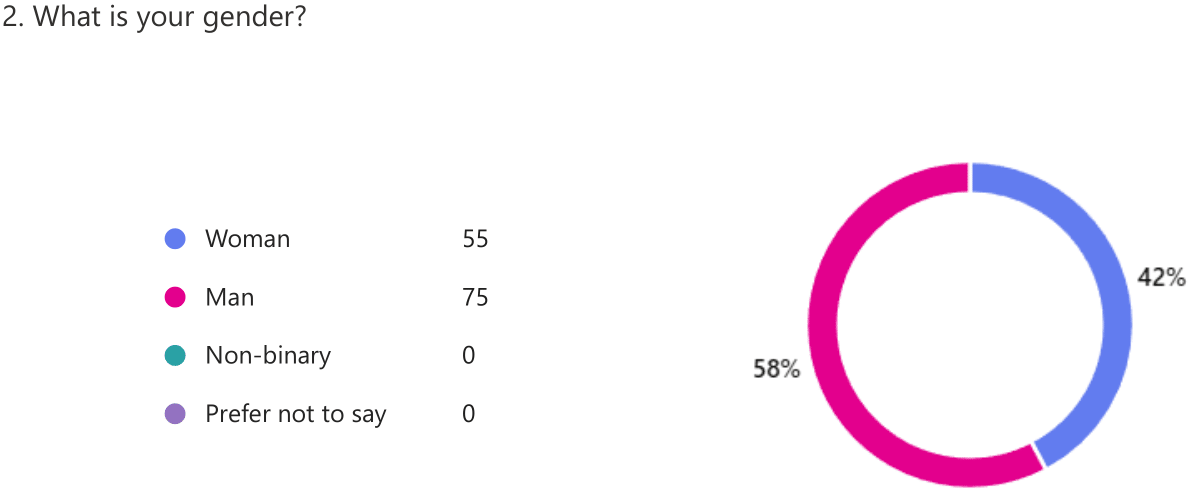
\includegraphics[width=\linewidth]{2}
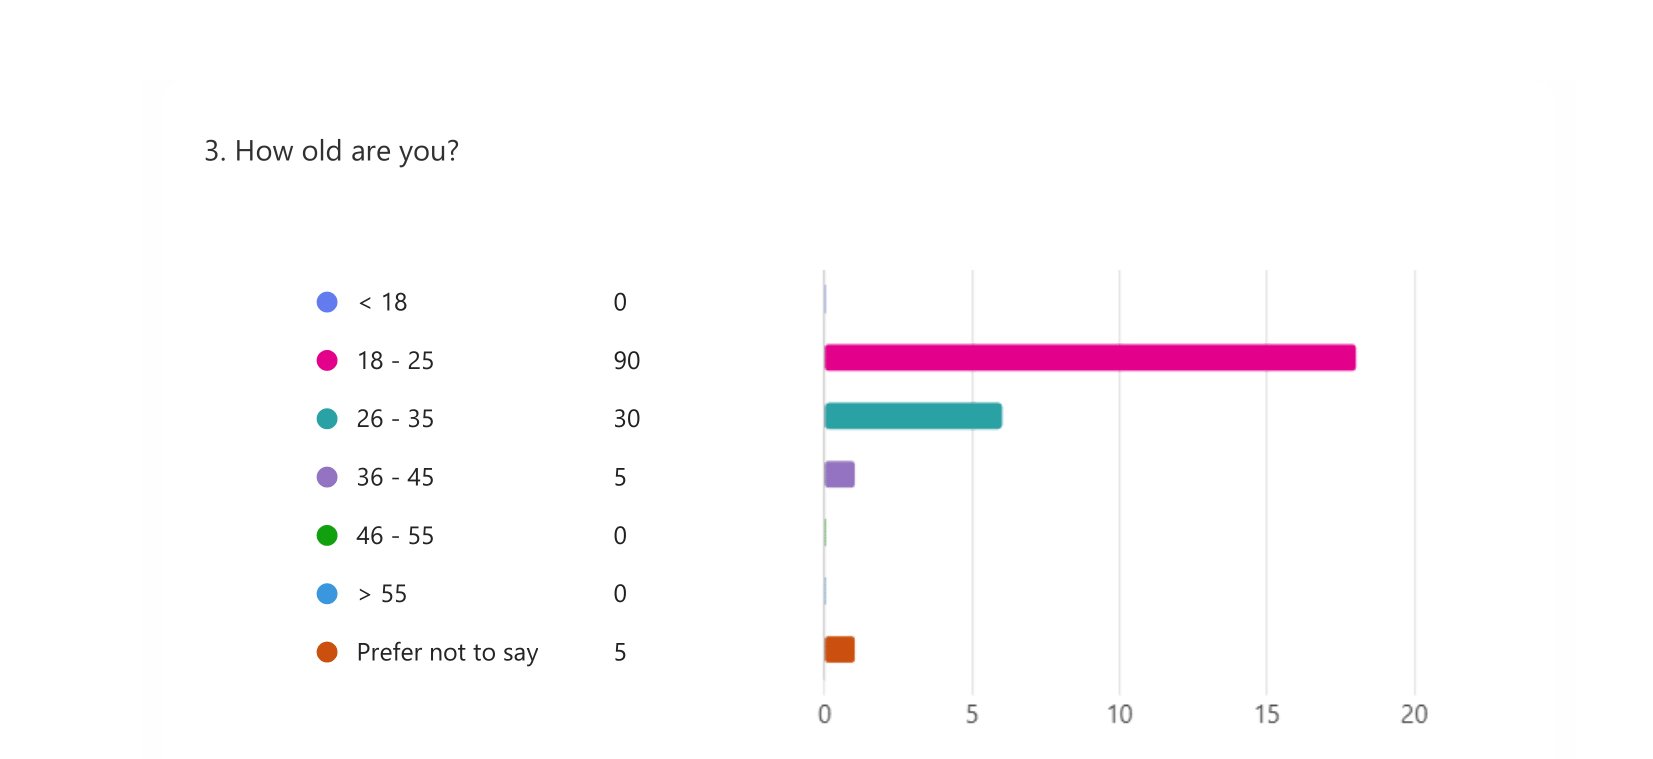
\includegraphics[width=\linewidth]{3}
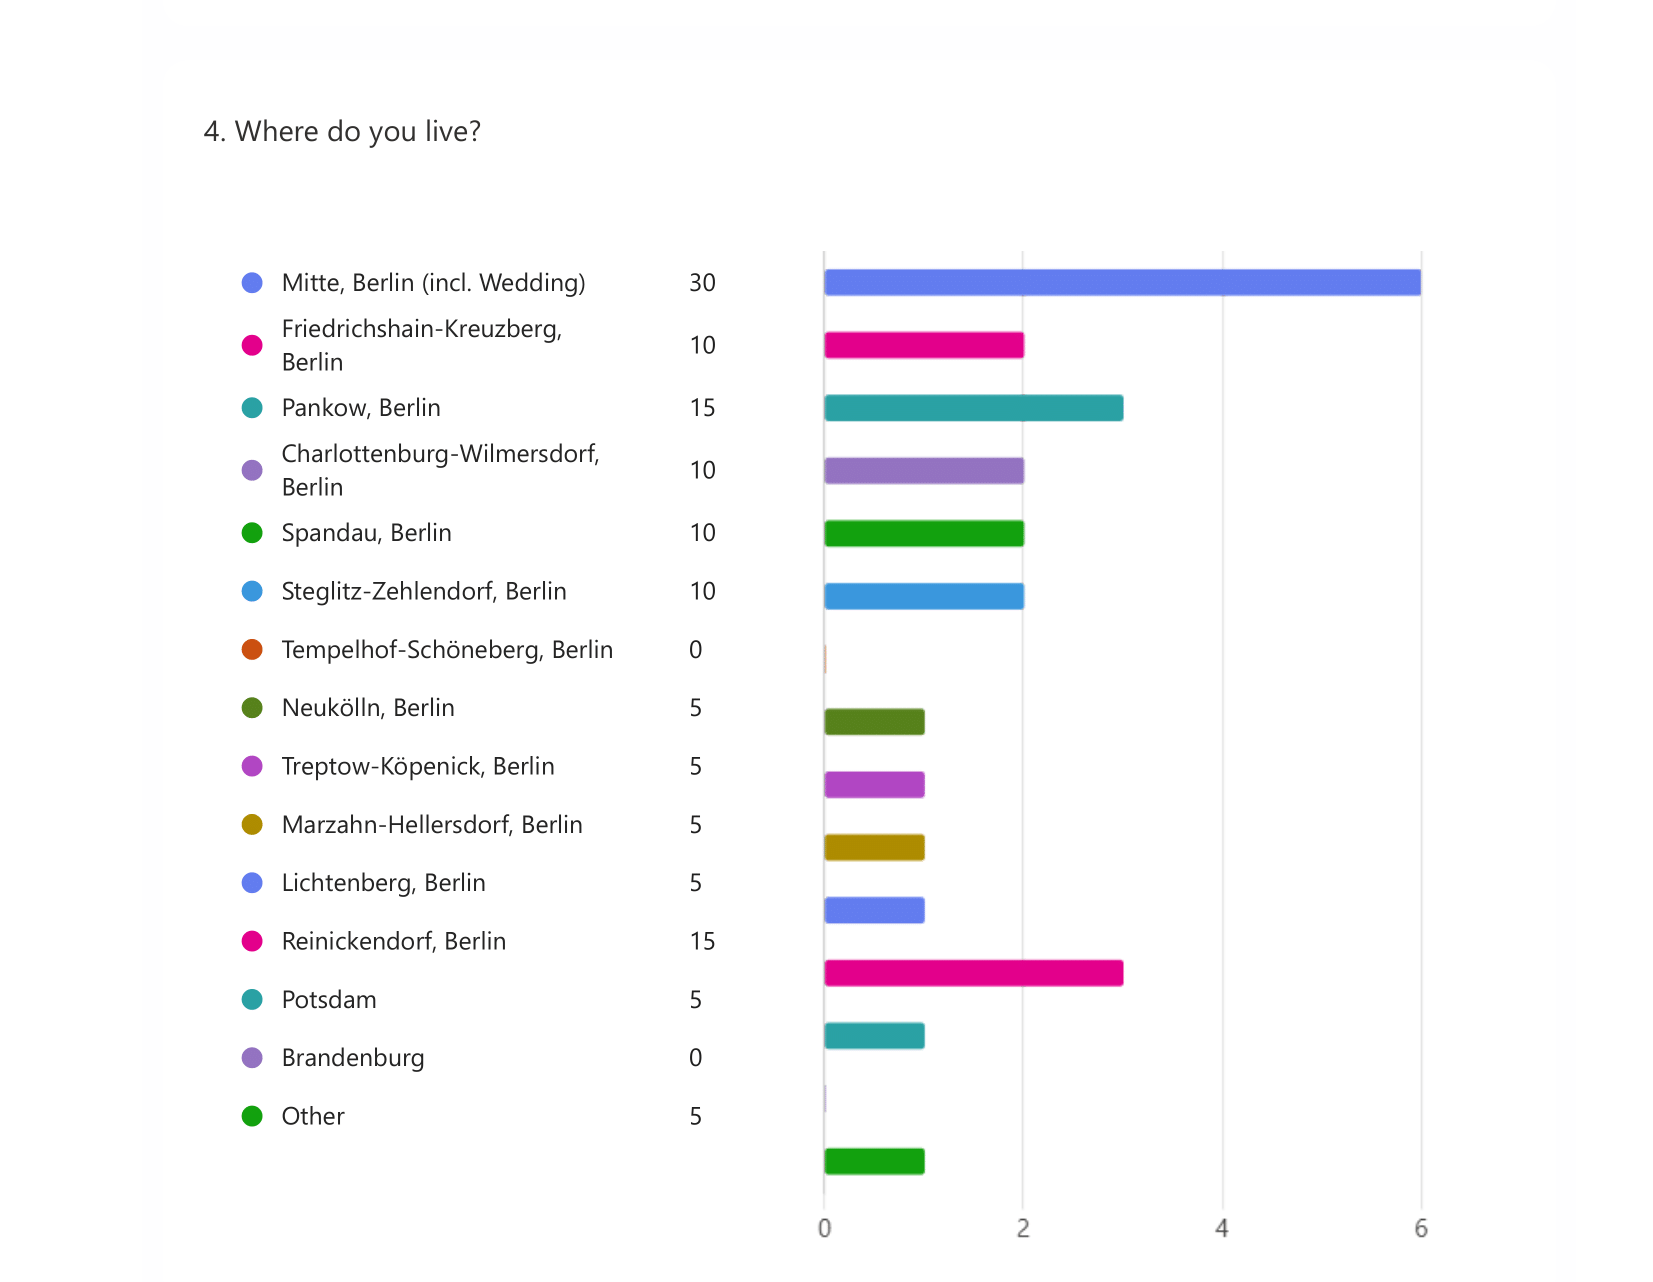
\includegraphics[width=\linewidth]{4}
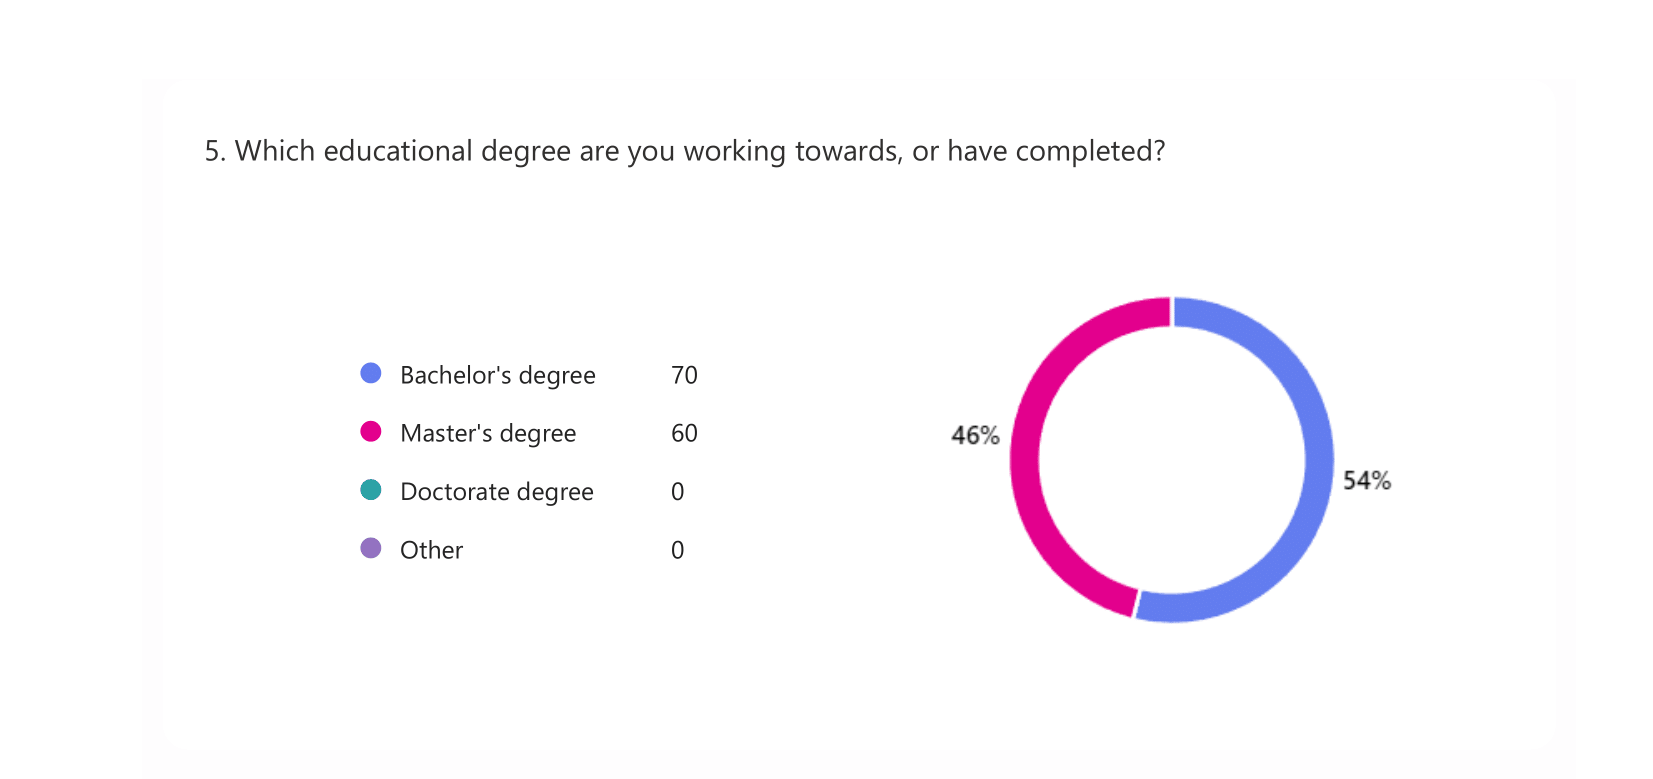
\includegraphics[width=\linewidth]{5}
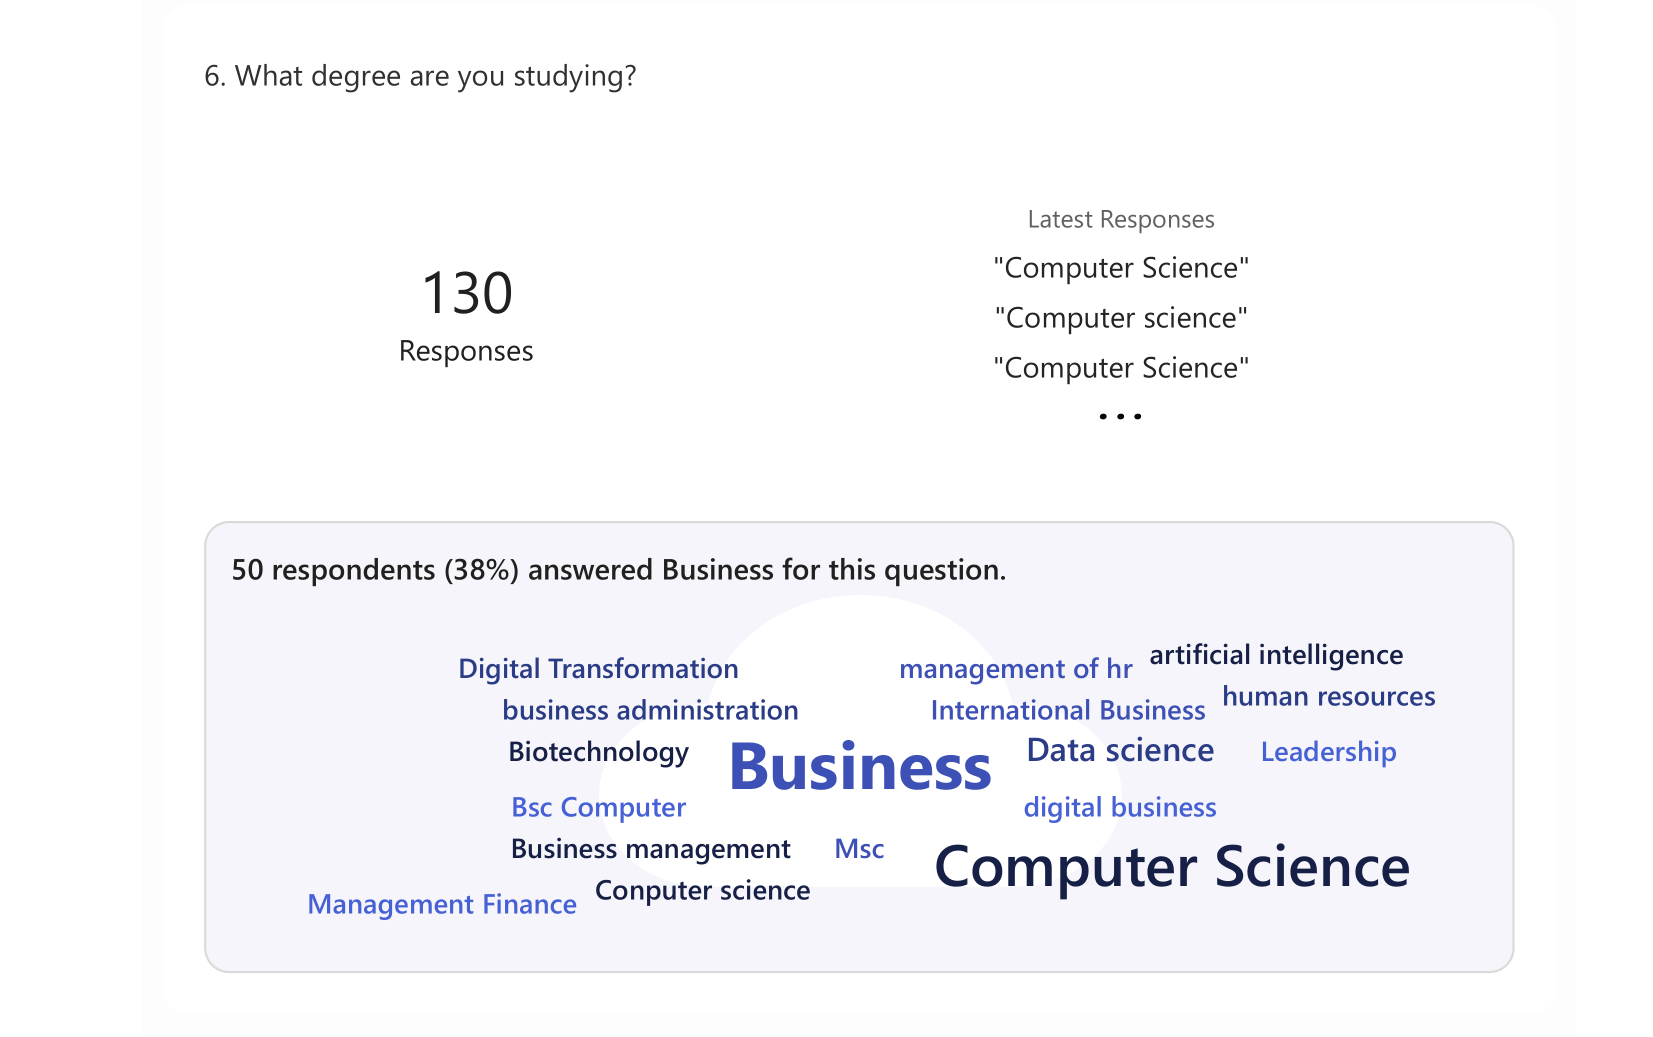
\includegraphics[width=\linewidth]{6}

\includegraphics[width=\linewidth]{7}
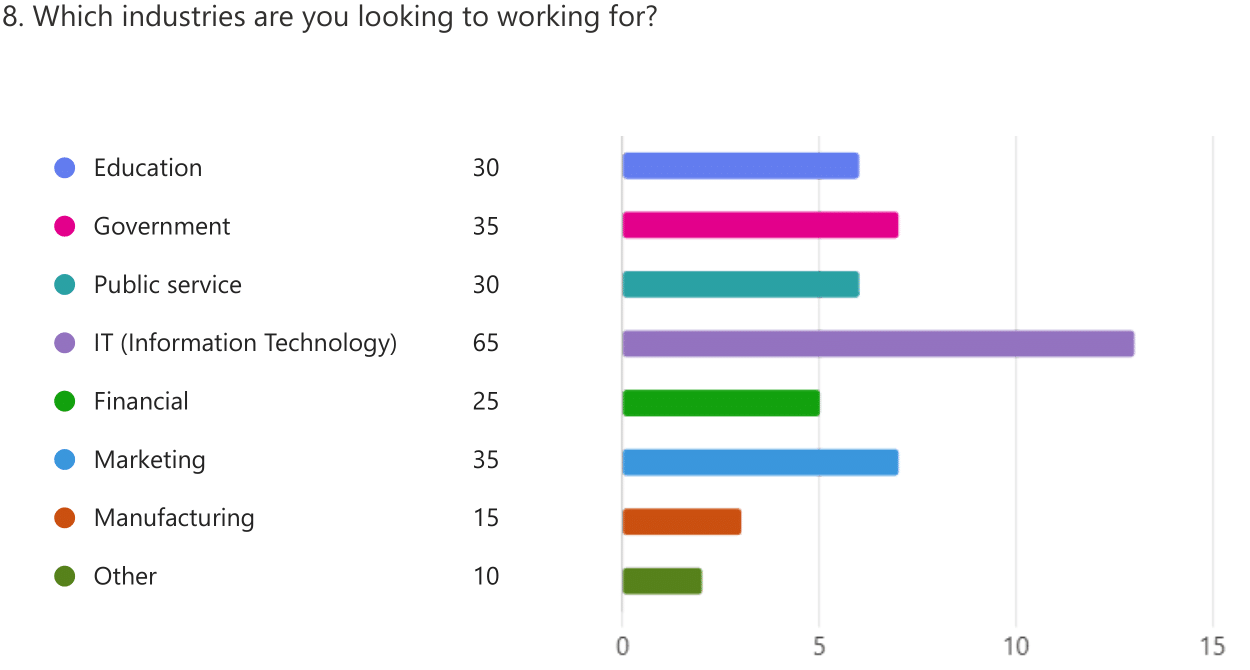
\includegraphics[width=\linewidth]{8}
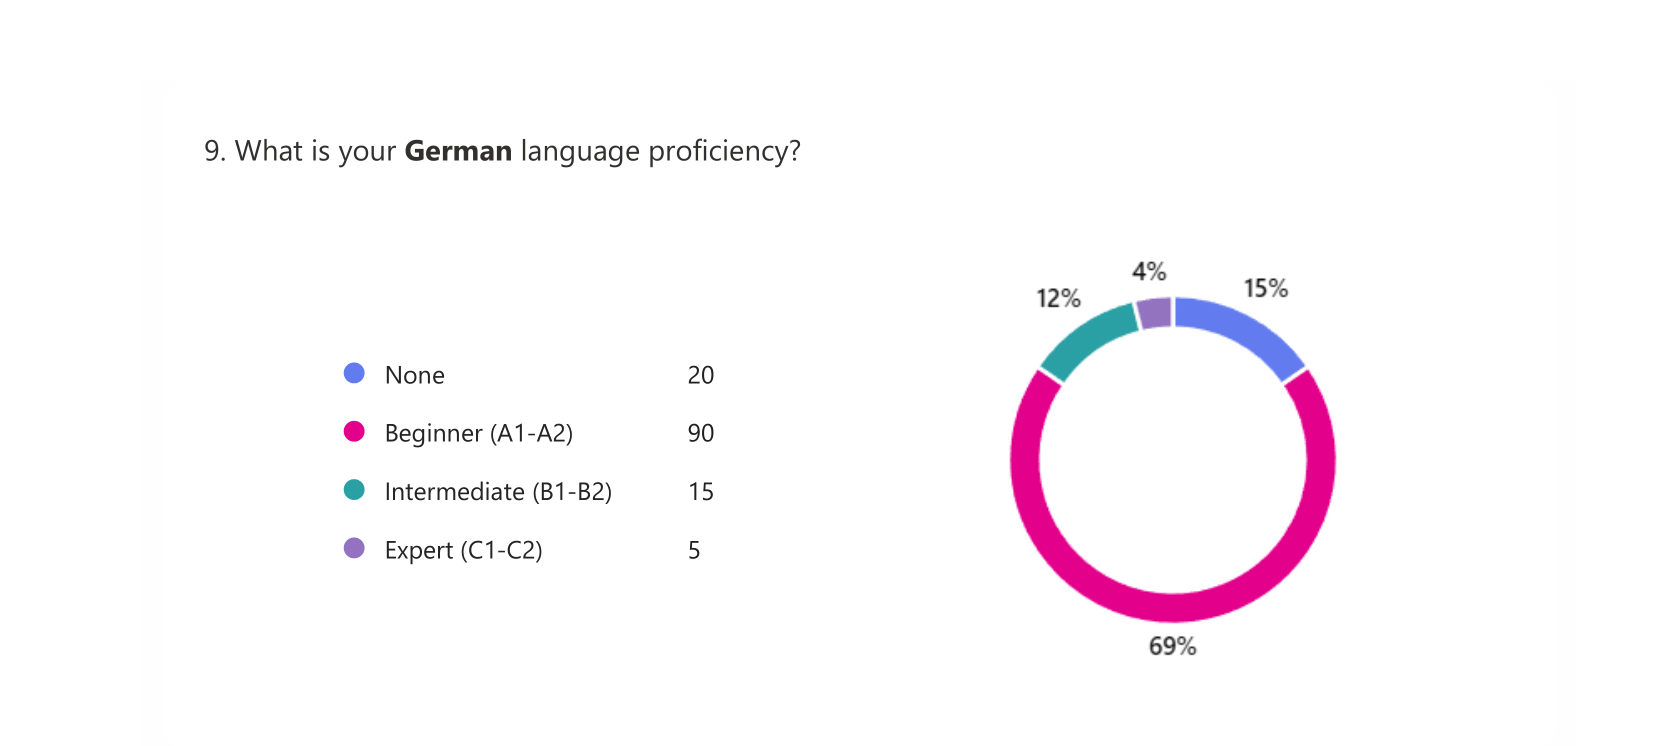
\includegraphics[width=\linewidth]{9}
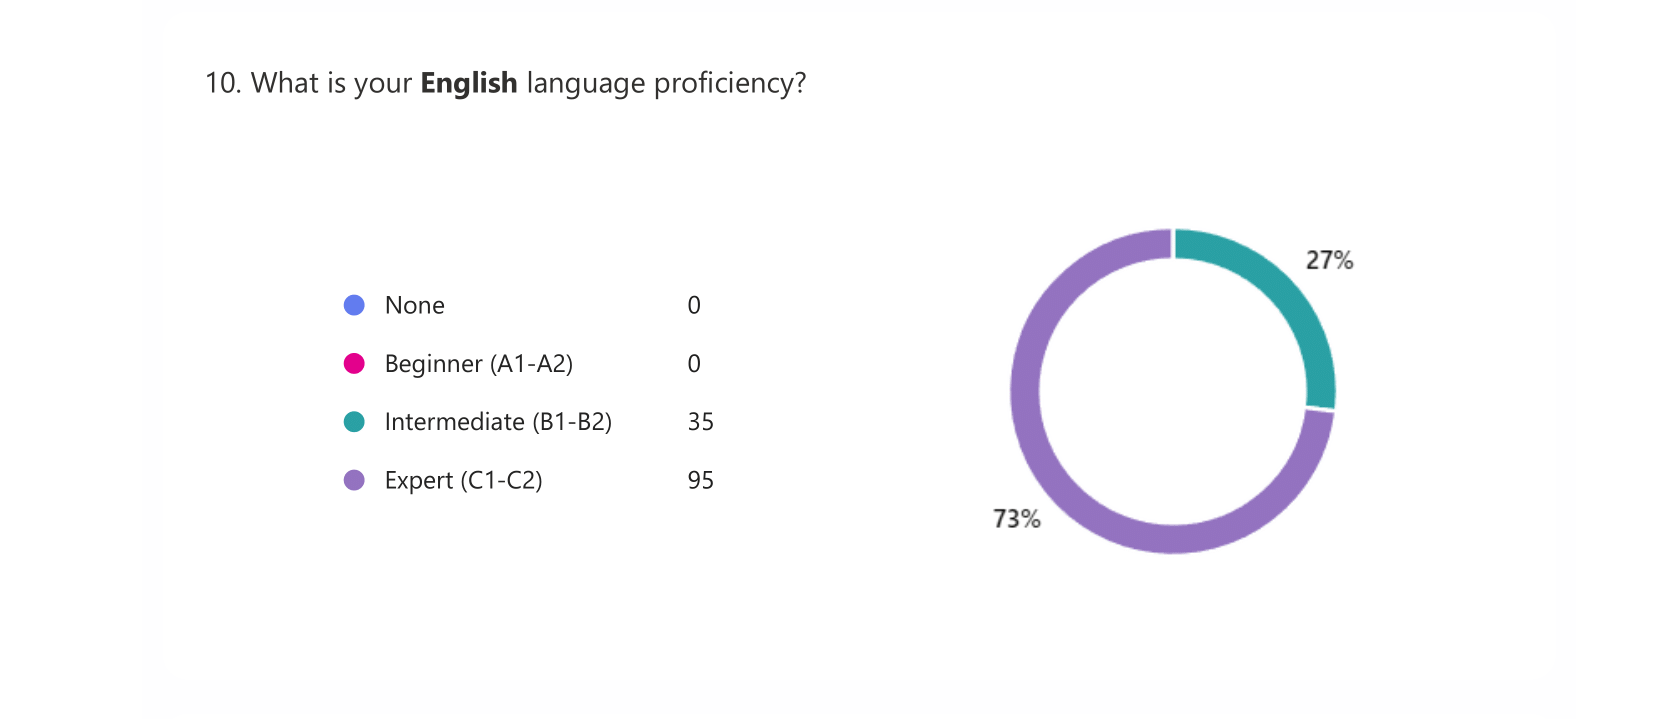
\includegraphics[width=\linewidth]{10}
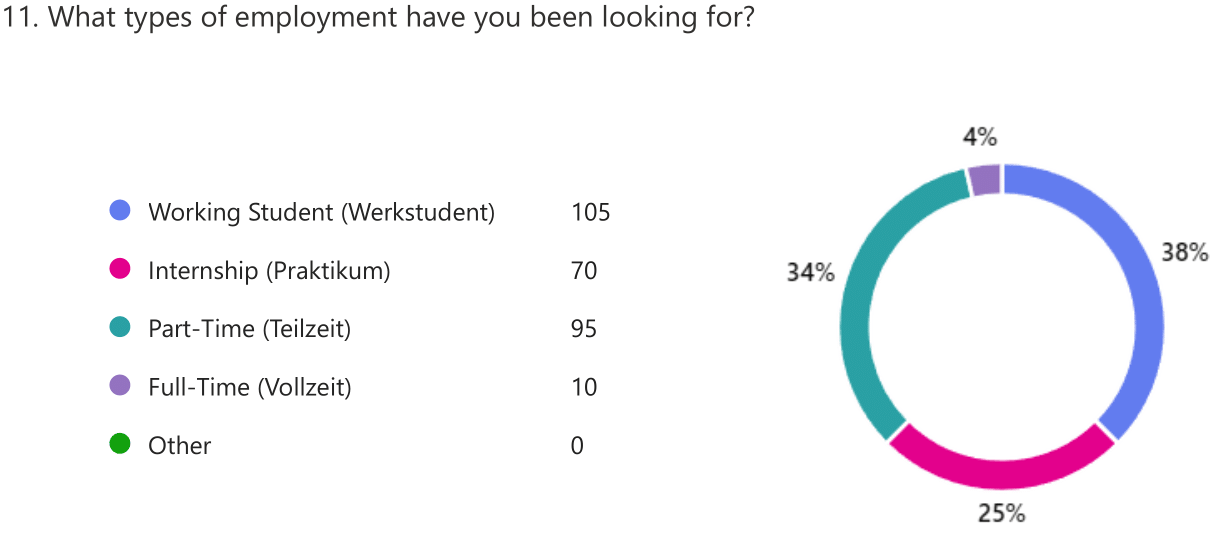
\includegraphics[width=\linewidth]{11}
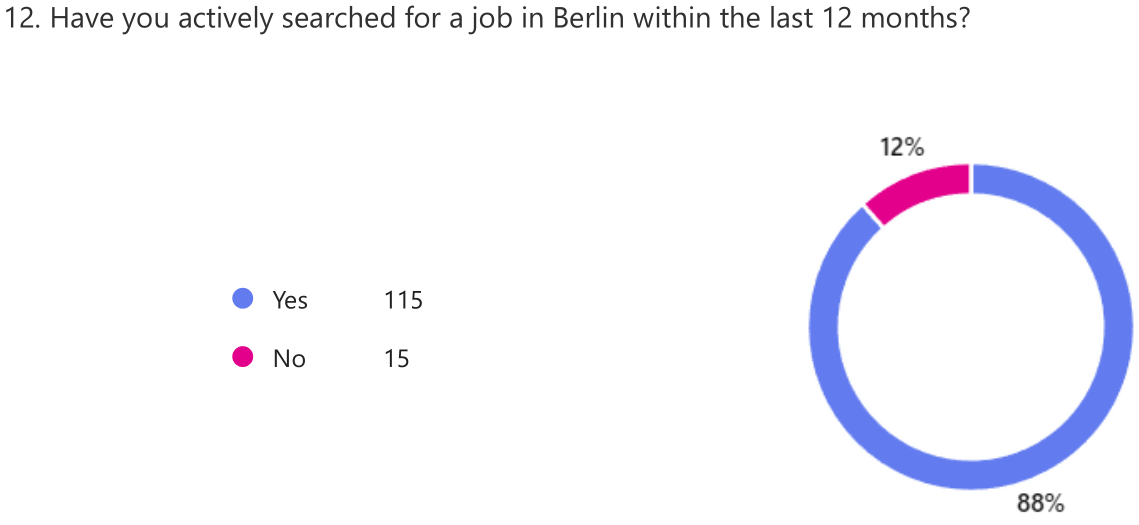
\includegraphics[width=\linewidth]{12}
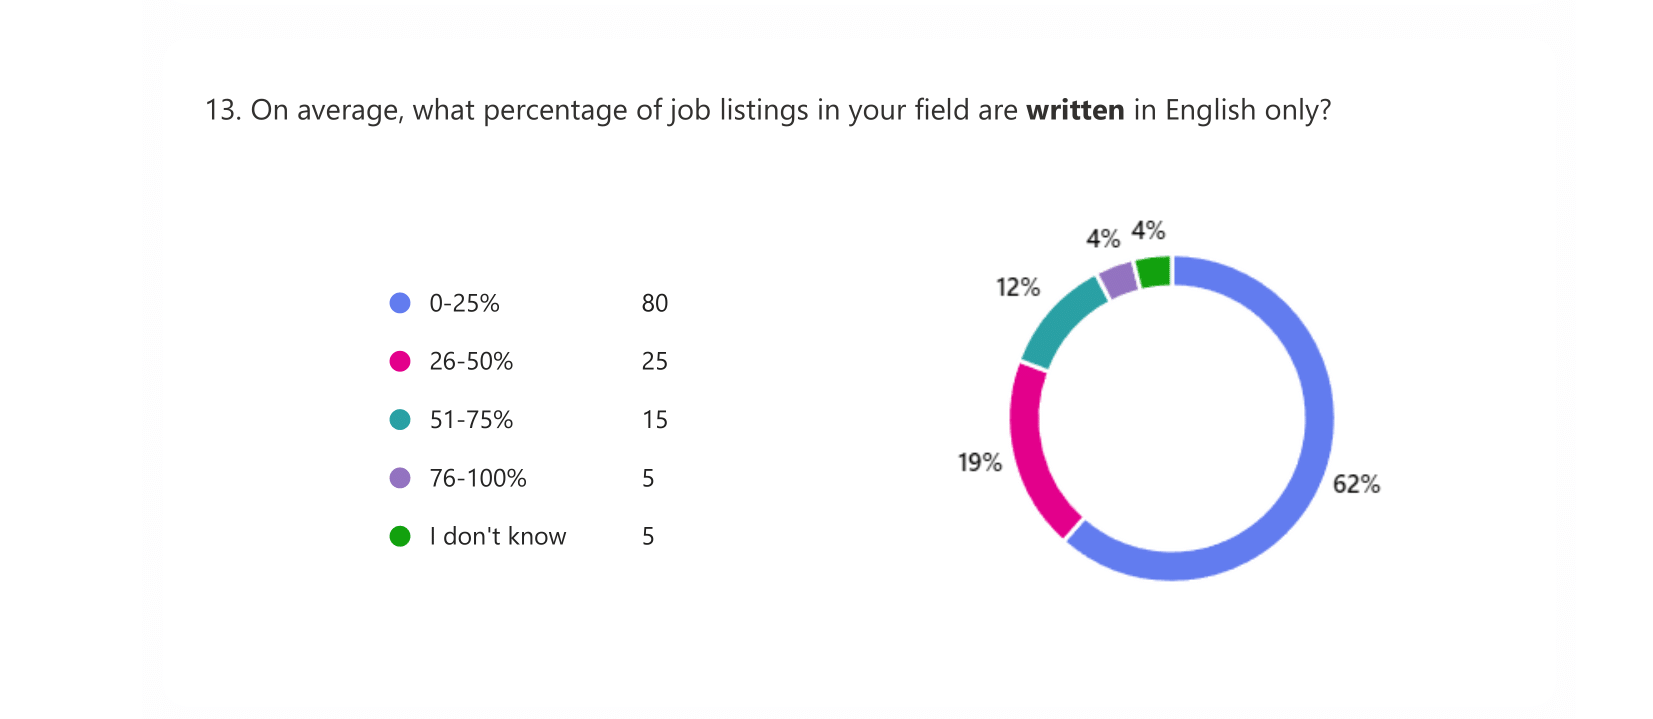
\includegraphics[width=\linewidth]{13}
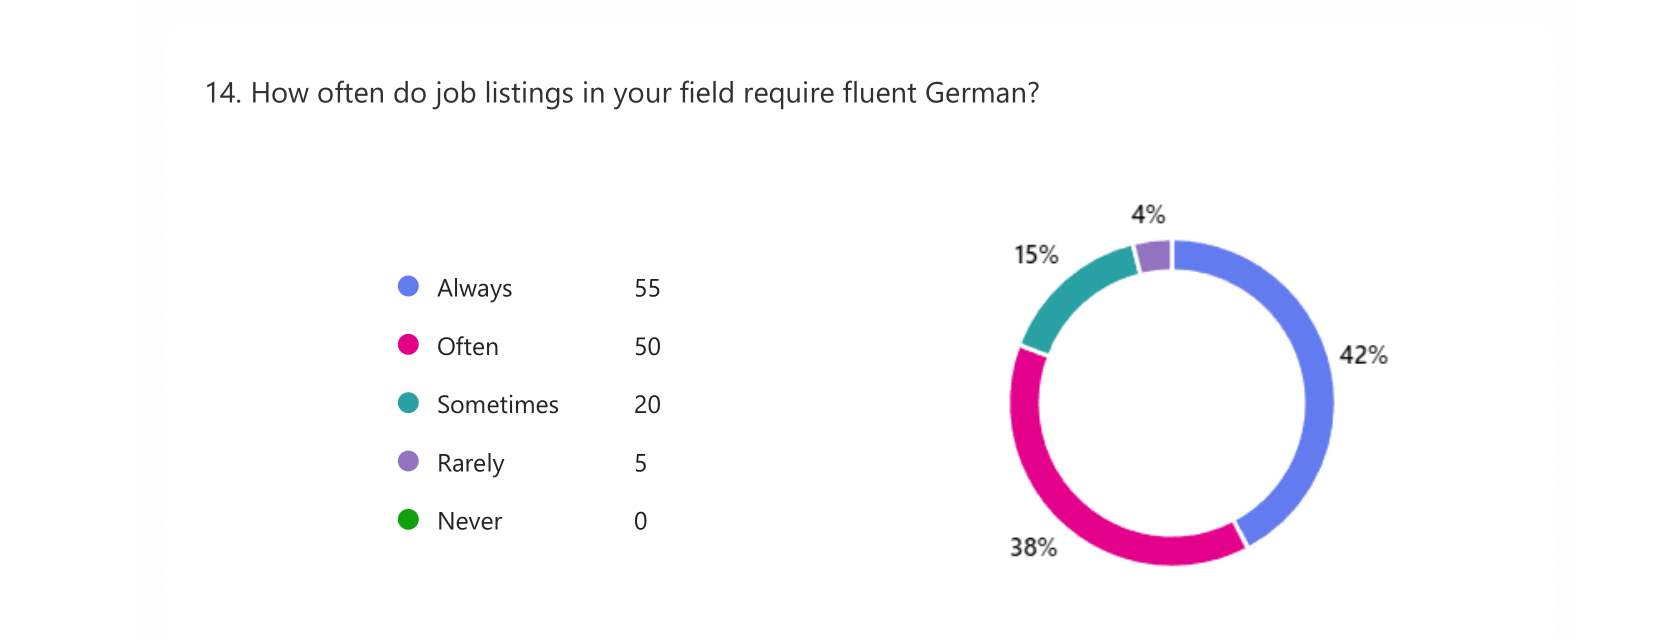
\includegraphics[width=\linewidth]{14}
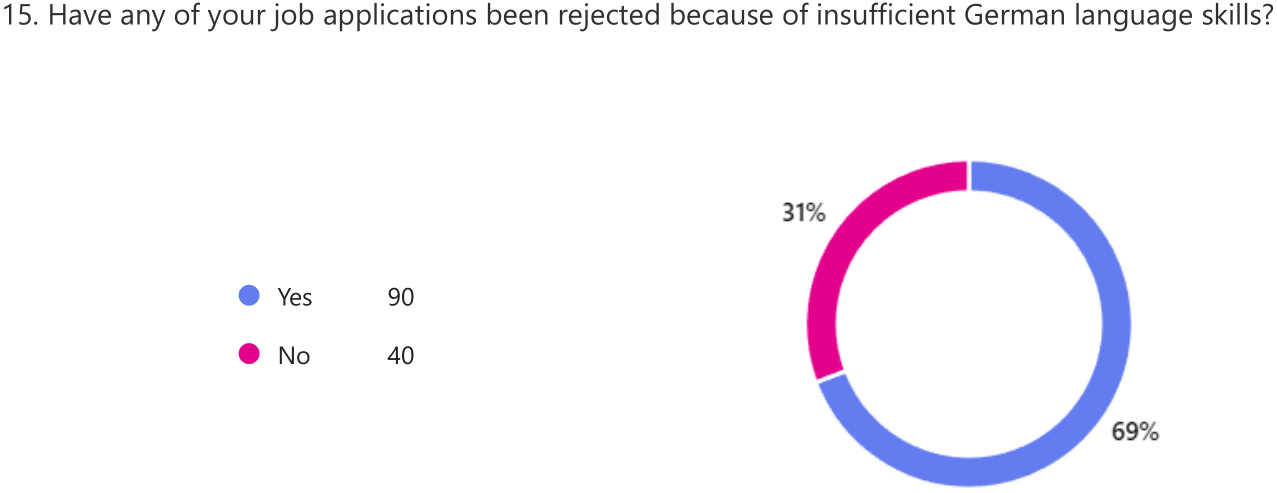
\includegraphics[width=\linewidth]{15}
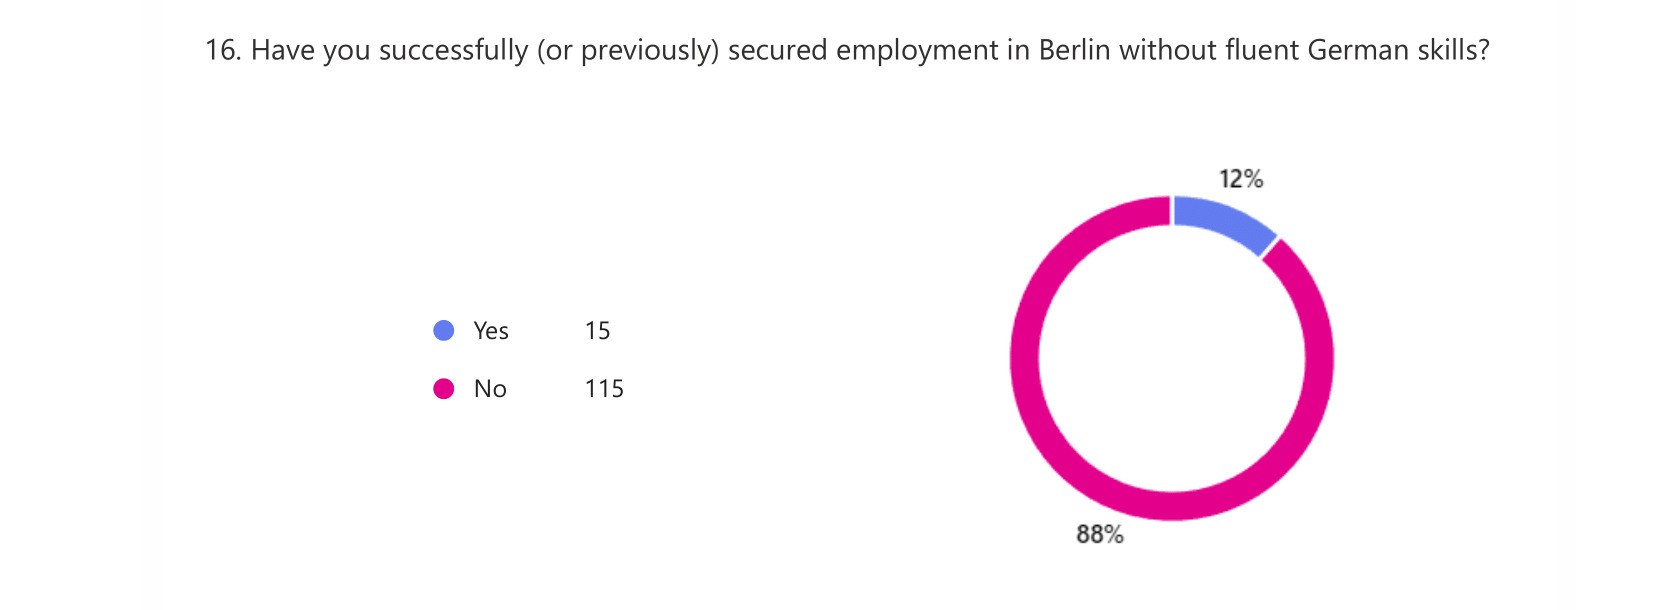
\includegraphics[width=\linewidth]{16}

\includegraphics[width=\linewidth]{17}
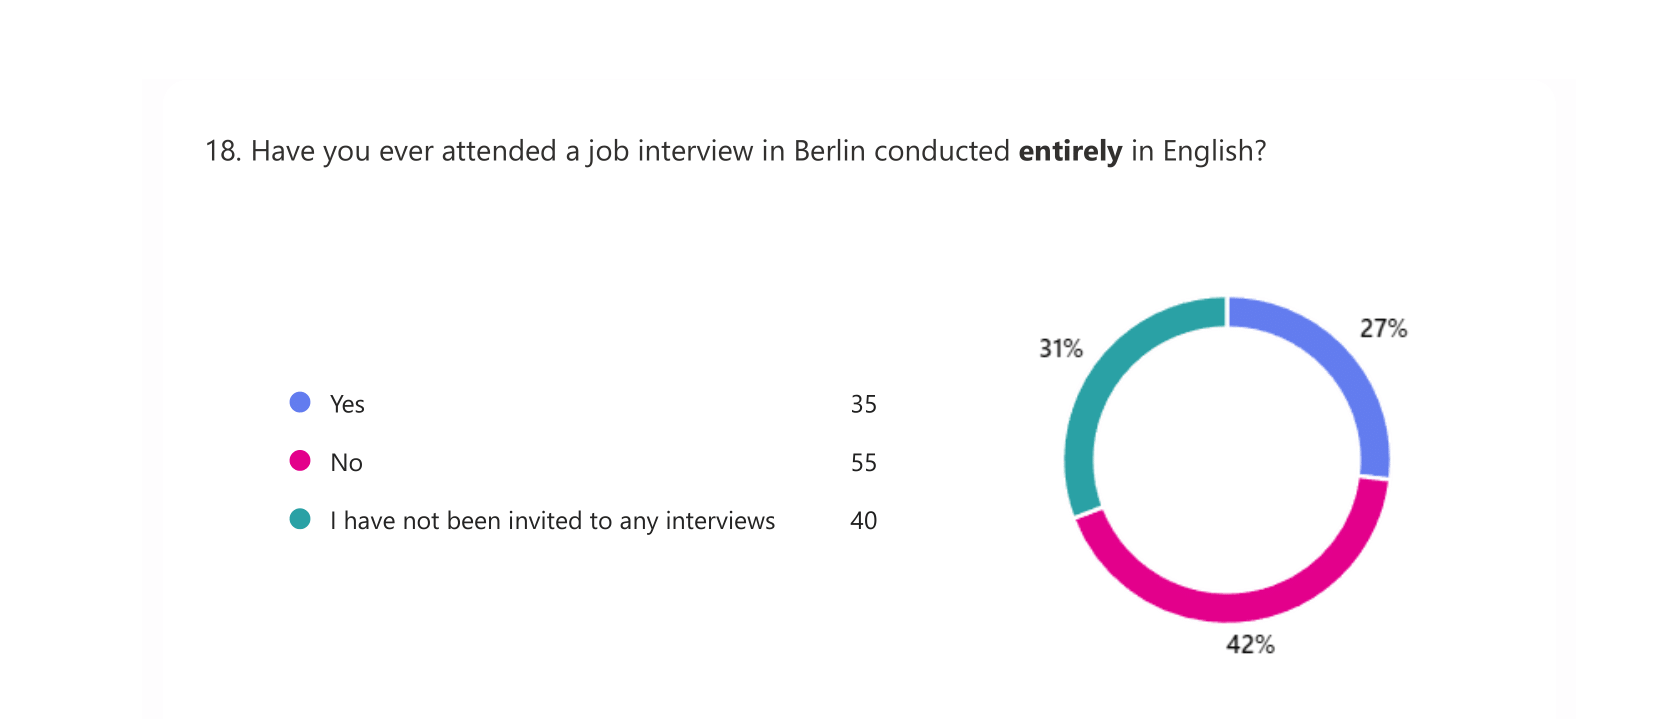
\includegraphics[width=\linewidth]{18}
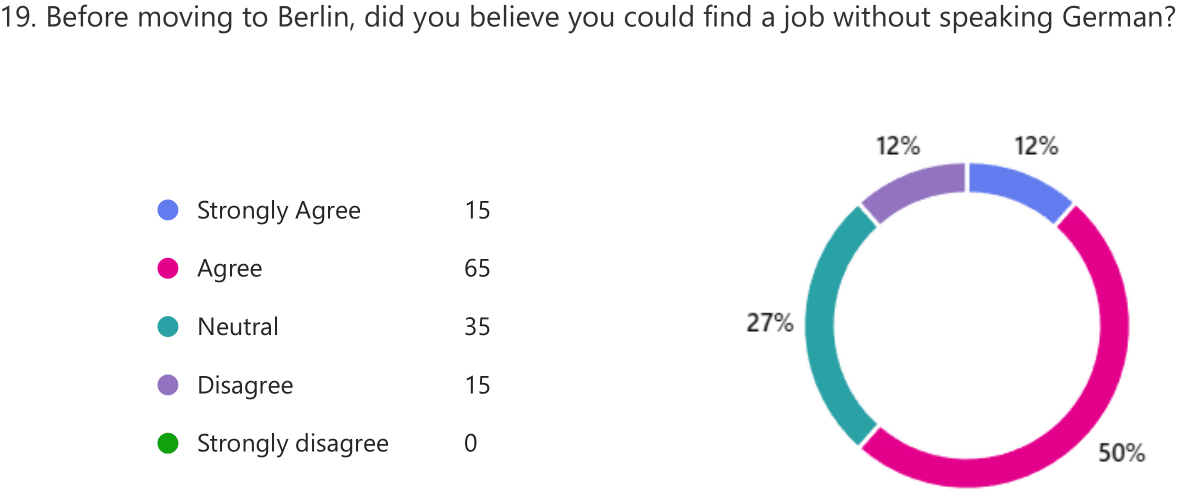
\includegraphics[width=\linewidth]{19}
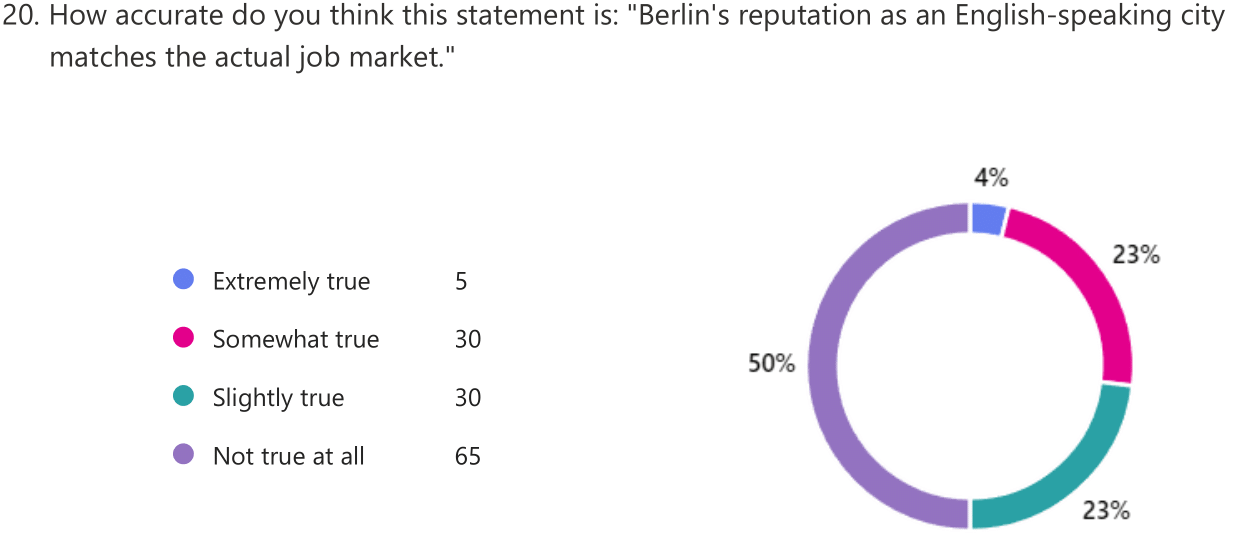
\includegraphics[width=\linewidth]{20}
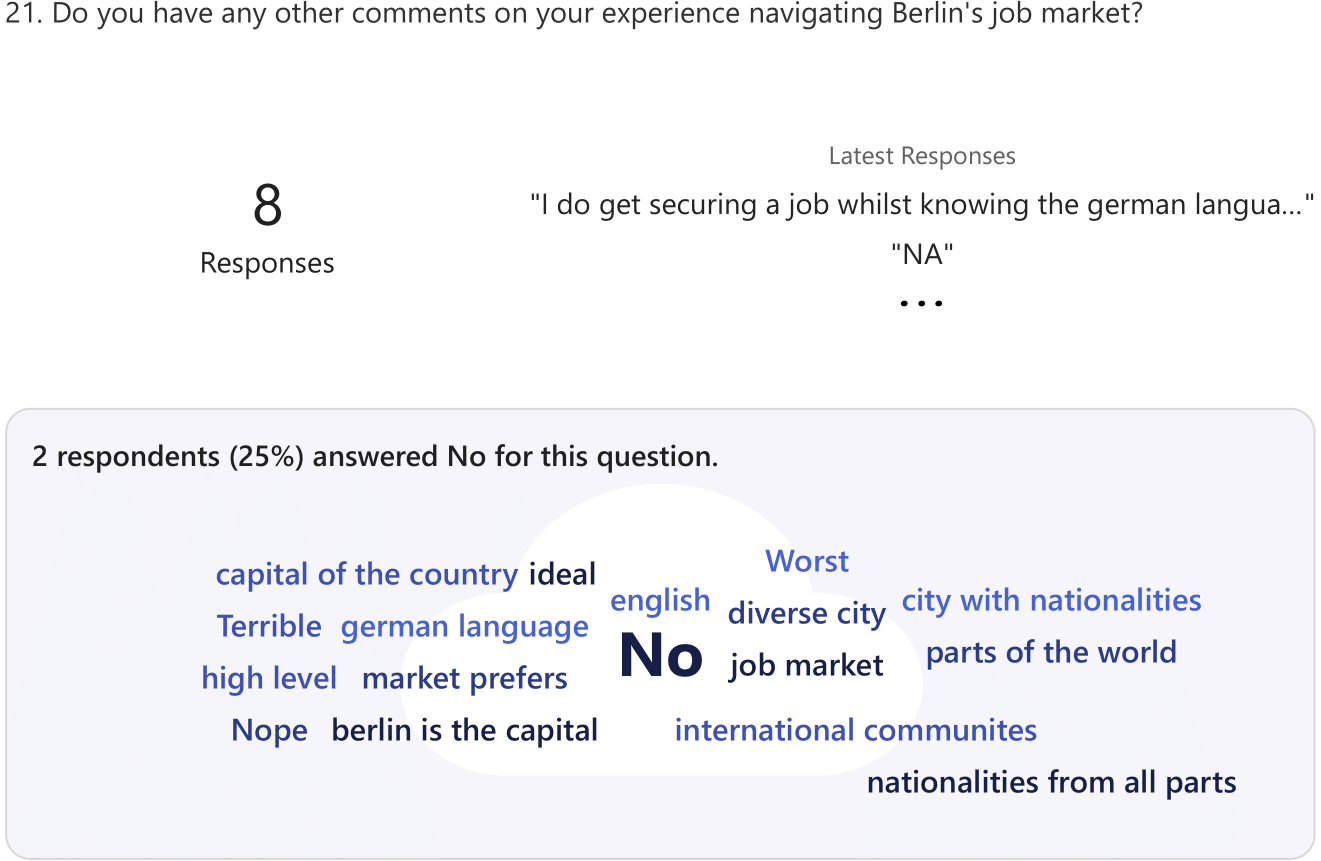
\includegraphics[width=\linewidth]{21}

\justifying
\clearpage
\section{Appendix B: Job Listing Analysis}
\label{appendix:B}
\vspace*{1em}
Reference the attached data collection file: \url{https://gismauniversity-my.sharepoint.com/:b:/g/personal/alimohamed\_fathi\_gisma-student\_com/Ea3b7Gcz0ZxMjmGRPkS7O6EBelOs1u99uhj4IqmTmiXyiQ?e=lzXTpU} \\

%or, alternatively, the Excel file: \url{https://gismauniversity-my.sharepoint.com/:x:/g/personal/alimohamed\_fathi\_gisma-student\_com/EU8FRhBpHQZEn8\_c8DtfuUEBunNnZHYwtcLO8X16ss4I4A?e=lLAXAV}

\graphicspath{ {./attachments/appB} }
\noindent
\section*{German Language Proficiency Level Required} \vspace{1em}

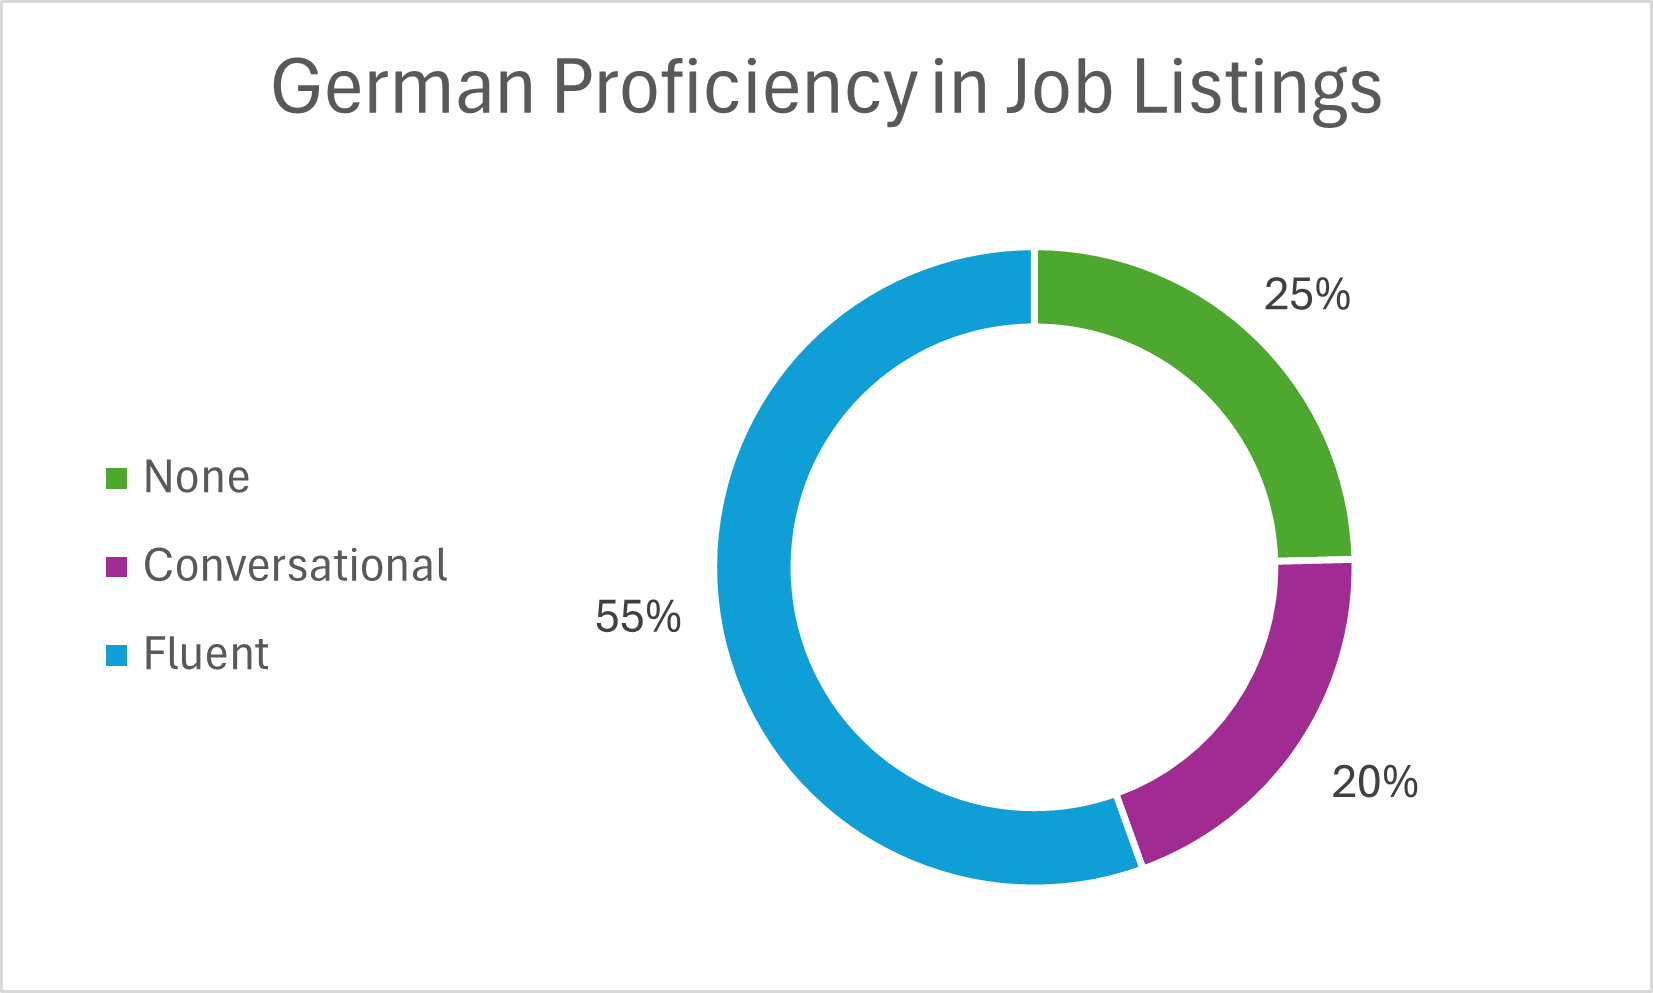
\includegraphics[width=\linewidth]{proficiencies}

\section*{Listing Languages} \vspace{1em}

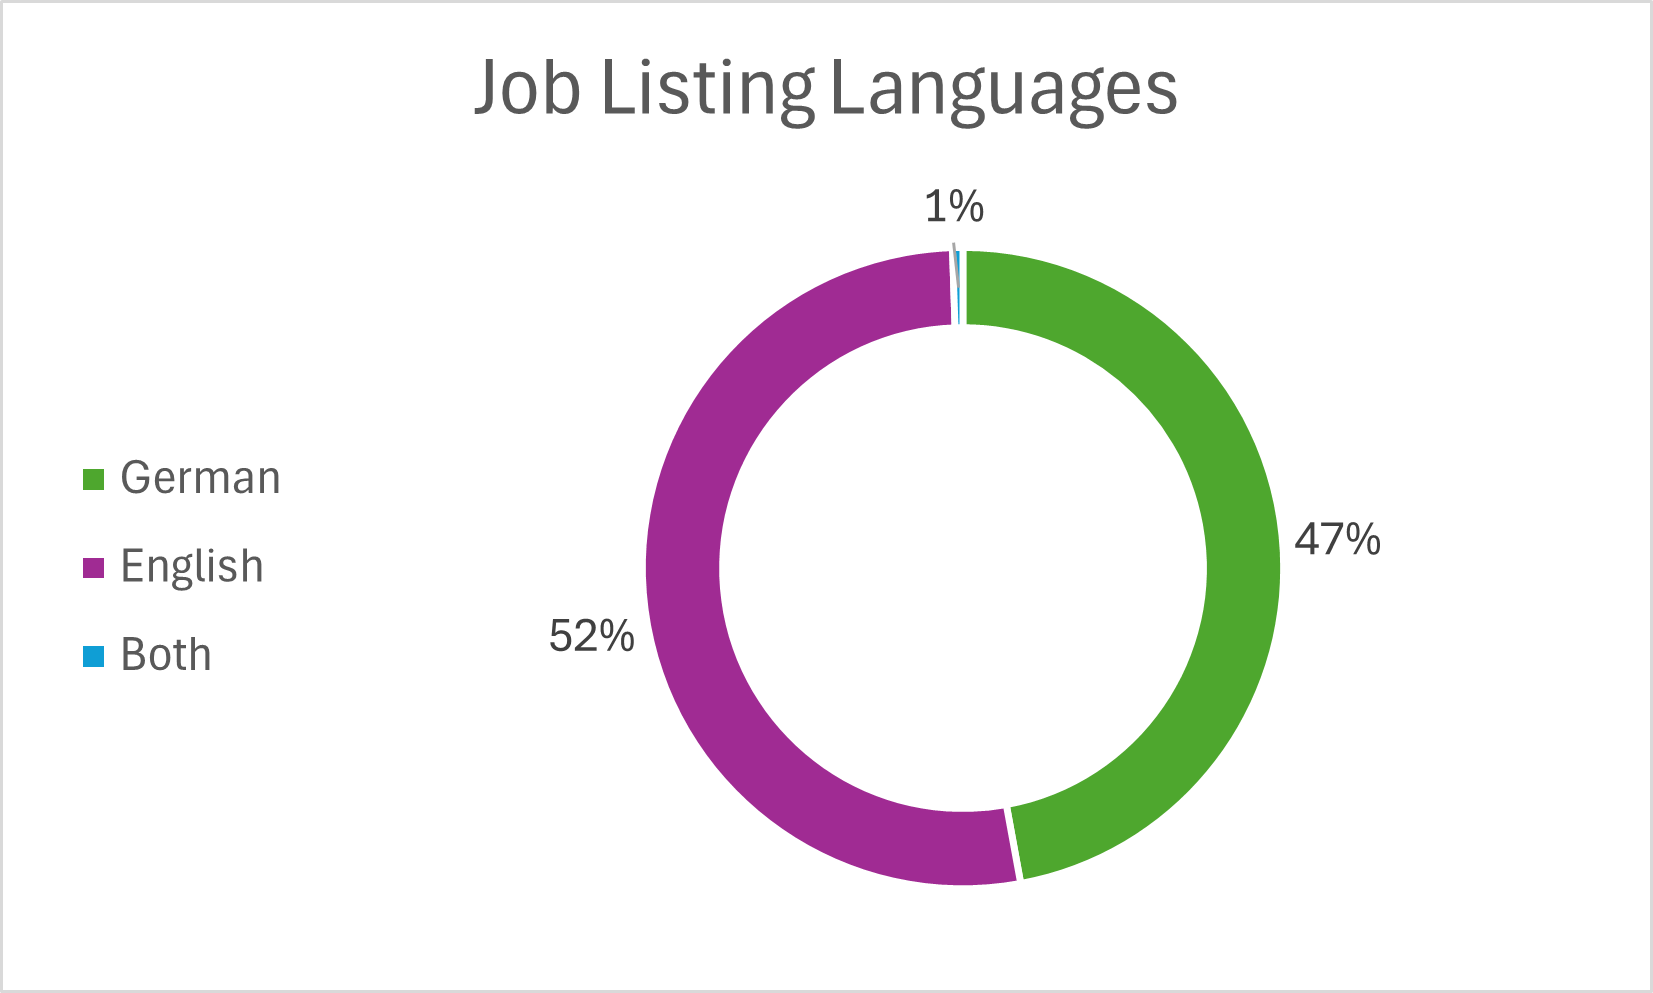
\includegraphics[width=\linewidth]{listinglangs}

\clearpage

%%%%%%%%%%%%%%%%%%%%%%%%%%%%%%%%%%%%%%%%%%%%%%%%%%%%
\end{document}
%%%%%%%%%%%%%%%%%%%%%%%%%%%%%%%%%%%%%%%%%%%%%%%%%%%%